%
% IEEE Transactions on Microwave Theory and Techniques example
% Tibault Reveyrand - http://www.microwave.fr
%
% http://www.microwave.fr/LaTeX.html
% ---------------------------------------



% ================================================
% Please HIGHLIGHT the new inputs such like this :
% Text :
%  \hl{comment}
% Aligned Eq. 
% \begin{shaded}
% \end{shaded}
% ================================================



\documentclass[journal]{IEEEtran}

%\usepackage[retainorgcmds]{IEEEtrantools}
%\usepackage{bibentry}  
\usepackage{xcolor,soul,framed} %,caption

\colorlet{shadecolor}{yellow}
% \usepackage{color,soul}
\usepackage[pdftex]{graphicx}
\graphicspath{{../pdf/}{../jpeg/}}
\DeclareGraphicsExtensions{.pdf,.jpeg,.png}

\usepackage[cmex10]{amsmath}
%Mathabx do not work on ScribTex => Removed
%\usepackage{mathabx}
\usepackage{array}
\usepackage{mdwmath}
\usepackage{mdwtab}
\usepackage{eqparbox}
\usepackage{url}

\hyphenation{op-tical net-works semi-conduc-tor}

%\bstctlcite{IEEE:BSTcontrol}


%=== TITLE & AUTHORS ====================================================================
\begin{document}
\bstctlcite{IEEEexample:BSTcontrol}
    \title{Modelo SIR - Python}
  \author{Manuel Deaza - 94412,~\IEEEmembership{Student Member,~ECCI}\\% <-this % stops a space
  Juan Camilo Ropero Mandon - 66320,~\IEEEmembership{Student Member,~ECCI,}
  }
  


% The paper headers
\markboth{Modelo SIR - Pyhton, SEPTIEMBRE~2022
}
{Roberg 
\MakeLowercase{\textit{et al.}}: High-Efficiency Diode and Transistor Rectifiers}


% ====================================================================
\maketitle



% === ABSTRACT ====================================================================
% =================================================================================
\begin{abstract}

The next article will present a littel simulation of SIR model using python, the model will present is based on the article "Mathematical models for economic evaluation: dynamic models based on differential equations", this article speak about spanish complaint and make a previous simulation using Mathematica software.
%\boldmath
\end{abstract}


% === KEYWORDS ====================================================================
% =================================================================================
\begin{IEEEkeywords}
Dynamic models, Infectious diseases, Differential equations, Economic evaluation, Data Science.
\end{IEEEkeywords}






% For peer review papers, you can put extra information on the cover
% page as needed:
% \ifCLASSOPTIONpeerreview
% \begin{center} \bfseries EDICS Category: 3-BBND \end{center}
% \fi
%
% For peerreview papers, this IEEEtran command inserts a page break and
% creates the second title. It will be ignored for other modes.
\IEEEpeerreviewmaketitle


% ====================================================================
% ====================================================================
% ====================================================================

% === I. INTRODUCTION =============================================================
% =================================================================================
\section{Introducción}
Se requiere realizar el modelado epidemiológico de una infección "x" a su vez es necesario actualizar y presentar dicha información en un cliente web 24/7 al servicio de algún usuario, dónde cada día según el comportamiento de la infección se realizan cambios en la información presentada además de re-estimar el modelo, una problemática que con Python se puede solucionar, más específicamente con librerías cómo Scipy para la aproximación analítica como también el modelado matemático y Djnago para generar el cliente web estructurado por un frontend y backend \cite{djnago}, desde donde se podrá acceder a la información desde cualquier navegador, esto se puede montar como servicio en la nube para estimaciones epidemiológicas expandiendo no solo la capacidad de acceso si no la potencia computacional que a nivel de usuario es algo insignificante pero a nivel ingeniería es una muestra detallada de los avances actuales y lo que vamos a nivel de procesamiento computacional.
A continuacion se presentara una solución con herramientas libres y con muchas posibilidades de expansión si el ingenio humano y Python da la posibilidad.
 
Basado en el texto \textbf{Modelos matemáticos para la evaluación económica: los modelos dinámicos
basados en ecuaciones diferenciales} se realiza el modelado del sistema de ecuaciones diferenciales no lineal presentado en el mismo con ayuda de Python, en el articulo se tiene como finalidad representar la gripe española con base en el modelo SIR y sus incidencias económicas con relación al uso de una vacuna posterior a ello se presentan los resultados obtenidos además de la discusión sobre la interpretación de los mismos \cite{articulo-sir}.

% === II. Harmonically-Terminated Power Rectifier Analysis ========================
% =================================================================================
\section{Modelo SIR}

Es un modelo epidemiológico simple que se usa para identificar características típicas de brote epidémicos, su fundamento es dividir la población infectada en grupos pequeños compartiendo ciertas características dependiendo el tipo de infección que se desarrolla \cite{modelo-sir-xd}.

Se clasifica en tres grupos importantes divididos en población susceptibles ($S$), infectada ($I$) y población recuperada o fallecida por esta infección ($R$).

Donde se determina una constante $N$ que se determina como  la población total en el modelo o $N=S+I+R$, para plantear las ecuaciones del modelo es necesario entender que se quiere determinar la velocidad de cada grupo poblacional en un determinado rango de tiempo, esta velocidad o cambio se entiende como la primera derivada, en base a esto se obtiene un sistema de ecuaciones que nos ayudara a aproximar un brote epidemiológico \cite{modelo-sir-tesis}:


\begin{equation}
\label{sistema_no_vacuna} 
\left\{
    \begin{array}{lr}
        S^\prime_{(t)} = -\beta S_{(t)} I_{(t)}\\
        I^\prime_{(t)} = \beta S_{(t)} I_{(t)} - yI_{(t)}\\
        R^\prime_{(t)} = yI_{(t)} 
    \end{array}
\right.
\end{equation}


Se puede identificar los valores de $\beta$ como la \textbf{tasa de contagio} y  $y$ como el \textbf{coeficiente retiro natural} \cite{articulo-sir}, la primera ecuación $S^\prime_{(t)}$ se determina como la velocidad de cambio de los susceptibles a otra población en su defecto infectados,
con el contacto entre susceptibles y infectados, se puede considerar estas dos variables en la hipótesis del modelo como directamente proporcionales además que acompañadas de una tasa de contagio conforman el grupo de susceptibles, a su vez es correcto determinar que los susceptibles infectados migraran a la segunda ecuación $I^\prime_{(t)}$ donde con base al coeficiente de retiro natural el cual se  multiplica con numero de infectados $y I_{(t)}$ se puede determina la velocidad de cambio de resistentes y recuperados $R^\prime_{(t)}$, además de ello el mismo factor disminuye la velocidad a la cual cambia los infectados $I^\prime_{(t)}$\cite{modelo-sir-xd}.

\section{Modelado Python}

Para realizar el modelo en Python se utilizo la librería \textit{Scipy} el cual con el modulo \textit{integrate} permite con el método \textbf{odeint(\textit{model(), y0, time})} solucionar sistemas de ecuaciones diferenciales de orden superior, este método utiliza un algoritmo escrito en FOORTRAN el cual hace uso del método Runge Kutta (RK)\cite{scipy-docs-odeint}, este método recibe como primer parámetro una función llamada \textbf{model(\textit{t,x,constantes})} la cual recibe como parámetros la variable independiente ($t$), la variable dependiente ($x$) junto con las constantes implicadas en el sistema; en esta función \textbf{model()} se deberá colocar el sistema de ecuaciones a solucionar o ecuación de orden superior como un sistema primer orden \cite{indu-sistema-primer-orden}, esta función debe retornara la derivada de cada función implicada en el sistema de ecuaciones diferenciales a modo de lista, suponiendo el modelo SIR se debera retornar una lista similar a \textbf{[dS, dI, dR]} donde $dS$ es la derivada de suceptibles o la razon de cambio de la poblacion suceptible en el tiempo, de igual manera $dI$ y $dR$, esto lo podemos ver mejor como: 

\begin{align*}
 [dS, dI, dR] &= [S^\prime_{(t)}, I^\prime_{(t)}, R^\prime_{(t)}] \\
 [dS, dI, dR] &= [-\beta S_{(t)} I_{(t)} , \beta S_{(t)} I_{(t)} - yI_{(t)} , yI_{(t)}]
\end{align*}

En el caso de el modelo a trabajar se tienen 3 funciones o variables $(S,I,R)$ importantes las cuales se desprenderán de la variable dependiente que pasamos en la función \textbf{model()}, esto asumiendo que la variable dependiente que se pase como parámetro la misma sera una lista donde se puede ubicar en cada posición de dicha lista las funciones implicadas en el sistema, en pocas palabras el parámetro $x$ en \textbf{model()} es una lista donde con de las 3 funciones en el sistema $S$ tomara la posición $x[0]$, la $I$ posición $x[1]$ y $R$ posición $x[2]$ \cite{modelado-python-EDO}.

Además de este parámetro el método \textbf{odeint()} para dar una solución requiere los valores iniciales de cada función en una lista $y0$, donde por ejemplo el valor inicial de dicha función $S$ en la posición 0 de $y0$ debe coincidir con la posición de $dS$ en la lista retornada por \textbf{model()}, además de estos valores iniciales recibe el tiempo de simulación o dominio el cual sera determinado como un arreglo \textit{numpy} con cada instante de tiempo a evaluar en el sistema, ahora es cuando entra el método de la librería numpy \textbf{linspace(inicio, fin, num-datos)}, este método recibe el limite inferior del dominio (inicio) seguido del limite superior (fin), acompañado también del numero de datos que se requieren en ese rango (num-datos), este método retorna un arreglo numpy con los valores solicitados \cite{numpy-linspace}.

Una vez con todos los parámetros listos se puede proceder a instanciar el método \textbf{odeint()}, este método retorna un conjunto de arreglos dentro de un arreglo, donde el arreglo en la posición 0 contempla los datos evaluados de cada una de las funciones o la solución aproximada a cada función, estos datos se devuelven también como lista, posteriormente se gráfica dichos valores con ayuda de \textit{matplotlib}, esta librería cuenta con el modulo \textit{pyplot} el cual posee el  método \textbf{plot(x,y)} este recibe como primer parámetro $x$ el cual son los datos en el eje independiente, el segundo parámetro ($y$) son los datos en el eje dependiente, estos dos parámetros mencionados pueden ser de tipo arreglo o escalar, ahora para generar un resultado con el método \textbf{show()} se da una visualización de la gráfica esperada, destacar que este plot se puede entender como un canva disponible para dibujar \cite{matplotlib-examples}.

Con lo anterior se procede a relacionar con el sistema de ecuaciones donde inicialmente se da los siguientes valores iniciales en el articulo, estos con base a datos del Centro Nacional de Epidemiología en España, aclarar que el tiempo que se tomara para la simulación es llamado \textbf{Año Epidemiológico de la gripe} (52 semanas) \cite{articulo-sir} este tiempo lo podemos ver gracias a numpy en un arreglo como $time = linspace(0,51,52)$
\begin{align*}
S_{(0)}&= 99986 \\
I_{(0)}&= 14 \\
R_{(0)}&= 0
\end{align*}

Además de esto en el articulo se llega a un valor de tasa de contagio $\beta$ igual a $\beta = 3.61x10^{-5}$ dato calculado en base al evento epidemiológico, además de ello el retiro natural $y$ que es un inverso del tiempo máximo de infección de un individuo en el articulo es determinado como $y = 3.47$ debido a que la gripe española en su máxima infección es de un periodo de 7 semanas \cite{articulo-sir}.

 En el articulo se relaciona una nueva función al modelo SIR original, el numero de vacunados \textbf{$V$} la cual se termina relacionando en el sistema como una disminución de susceptibles y aumento de resistentes, este numero esta determinado hipotéticamente por la siguiente relación \cite{articulo-sir}:

\begin{equation}
\label{vacunados}
        V = \frac{Nve}{9}
\end{equation}

donde $N$ se reconoce como el numero total de la población ya relacionado anteriormente, $v$ índice per capita de vacunación dado en el articulo como 0.20, $e$ el índice per capita de eficacia de la vacuna dado en el articulo como 0.67, estos índices son proporcionados en el articulo, todo esto sobre $9$ que es la duración en semanas de la campaña de vacunación, este tiempo es determinado en el articulo como el correcto para iniciar una mitigación, iniciando después de la semana 9 y finalizando en la 18, esto se puede ver como una función a trozos de $V$ donde solo se cuente el numero de vacunados en el tiempo definido para la campaña de vacunación (semana 9-semana 18), esto se puede ver como:

\begin{equation}
\label{funcion_trozos_vacunados}
V(t) = 
\left\{
    \begin{array}{lr}
        0,\text{ }\text{si } 0\leq t\leq9\\
        V,\text{ }\text{si } 9<t\leq 18\\
        0,\text{ }\text{si } 18<t\leq51
    \end{array}
\right.
\end{equation}

Ahora bien, como se requiere hacer un análisis con y sin vacuna, se determina un nuevo sistema con base al modelo SIR donde se relaciona la función $V_{(t)}$ con los suceptibles y resistentes, este sistema luce de la siguiente manera:

\begin{equation}
\label{sistema_vacuna} 
\left\{
    \begin{array}{lr}
        S^\prime_{(t)} = -\beta S_{(t)} I_{(t)} - V_{(t)}\\
        I^\prime_{(t)} = \beta S_{(t)} I_{(t)} - yI_{(t)}\\
        R^\prime_{(t)} = yI_{(t)} + V_{(t)}
    \end{array}
\right.
\end{equation}

En python se realizan dos modelos basados en la función \textbf{model()} uno para el sistema donde se cuenta el numero de vacunados y otro para el que no, estos están determinados por las funciones en el codigo \cite{codigo-articulo}  \textbf{modelWithVaccine(t, x, B, Y, N,v,e)} y sin vacuna \textbf{modelWithoutVaccine(t, x, B, Y)} donde comparten los parámetros básicos de \textbf{model()}, como lo es el tiempo, la variable dependiente y las constantes, rescatando que en el modelo con vacuna se encuentran las constantes para determinar el numero de vacunados ($e,v,N$) como parámetros, donde la función a trozos que representa $V$ vista en Python es un proceso de condicionado donde se evalúa cada instante de tiempo en simulación y se determina si hace efecto $V$ en las relaciones de \ref{sistema_vacuna} dependiendo de las condiciones definidas en \ref{funcion_trozos_vacunados}, estos modelos retornan un arreglo similar a \textbf{return [dS, dI, dR]} donde la primera posición es la derivada de la función $S$ que ya sabemos la equivalencia en \ref{sistema_no_vacuna} y \ref{sistema_vacuna} y de las demás derivadas de las funciones restantes, recordando que esta posición que tiene $dS$ en este arreglo la comparte en el arreglo de valores iniciales $y0$.

Estos dos modelos son solucionados en dos instancias del metodo \textbf{odeint()}, en el codigo \cite{} el objeto con la solución del modelo con vacuna se denota como \textbf{solutionWithVaccine} de igual manera el objeto con la solución del modelo sin vacuna es \textbf{solution}, cada uno de estos objetos tienen en sus propiedades la solución al sistema en caso tal (vacuna o no), estos modelos se rigen bajo las condiciones iniciales mencionadas, en codigo estas condiciones iniciales lucen como $y0 = [S0, I0, R0]$ donde $S0$ es el valor inicial de $S$, es importante visualizar que la posición 0 donde esta la función $S$ de $y0$ coincide con la posición del arreglo de derivadas retornado por el modelo tal.

\begin{figure}[h]
  \begin{center}
  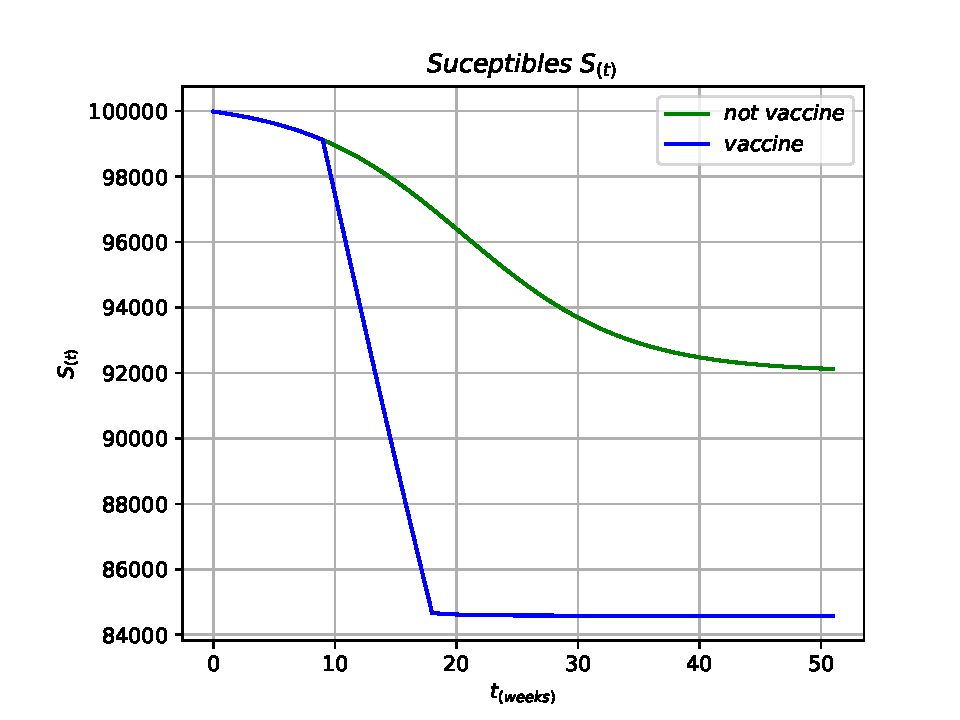
\includegraphics[width=3.3in]{pdf/suceptilbles.pdf}
  \caption{Velocidad cambio susceptibles en el tiempo, de linea azul modelado con vacuna y linea verde sin vacuna. }\label{sucepti-graf}
  \end{center}
\end{figure}

Una vez realizada la simulación con base al arreglo numpy \textbf{time} se realiza la representación gráfica de cada una de las funciones, en dicha gráfica se relaciona tanto con vacuna como sin vacuna, la gráficas que representa el cambio de susceptibles en el tiempo es Fig.\ref{sucepti-graf}, la de variación de infectados es Fig.\ref{infectad-graf} y la variación de recuperados o fallecidos es Fig.\ref{resis-graf}



\begin{figure}[h]
  \begin{center}
  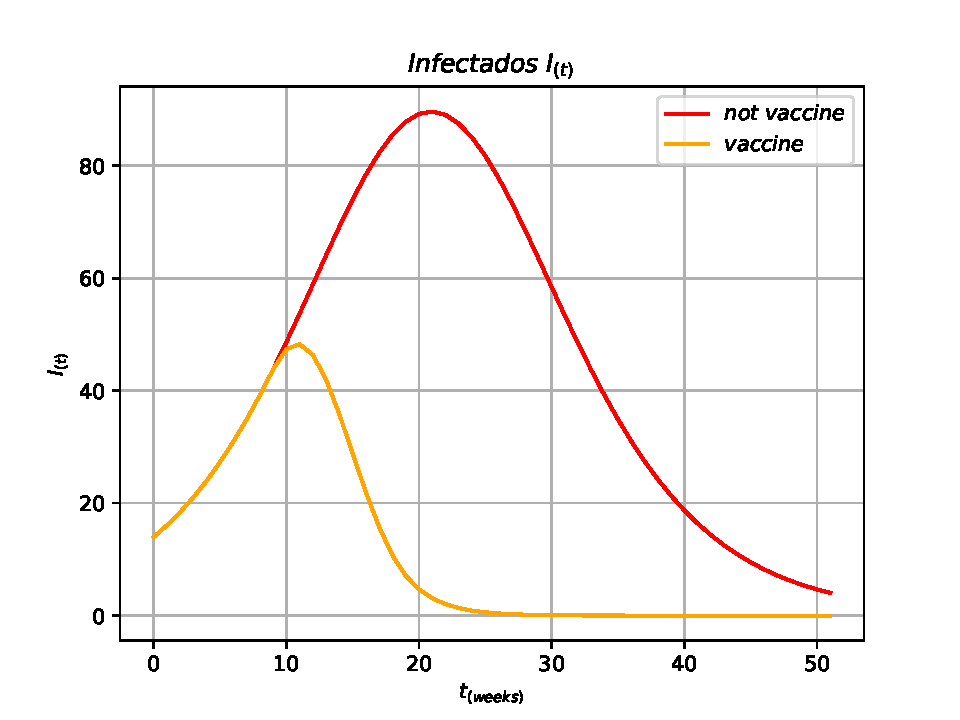
\includegraphics[width=3.3in]{pdf/infectados.pdf}
  \caption{Velocidad cambio infectados en el tiempo, de linea amarilla modelado con vacuna y linea naranja sin vacuna. }\label{infectad-graf}
  \end{center}
\end{figure}

De esta manera se logra modelar un sistema de ecuaciones en Python, importante tener claro que todo se fundamenta en la función \textbf{model()}, a continuación se discutirá acerca de los datos arrojados en las gráficas.

\begin{figure}[h]
  \begin{center}
  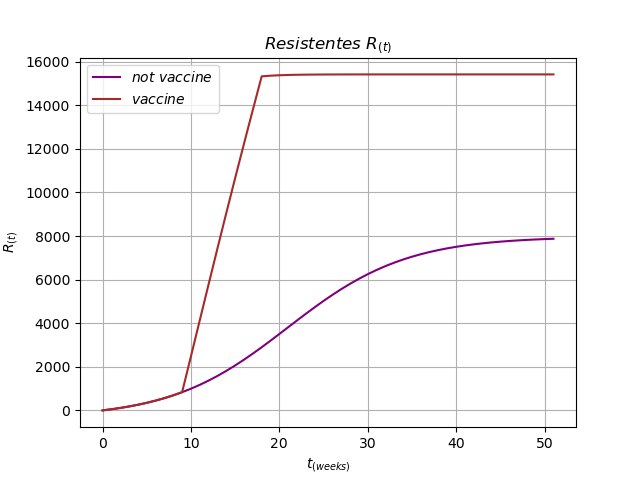
\includegraphics[width=3.3in]{photo/resistentes.png}
  \caption{Velocidad cambio resistentes en el tiempo, de linea cafe modelado con vacuna y linea purpura sin vacuna. }\label{resis-graf}
  \end{center}
\end{figure}

\section{Discusión}

Se concluye que mediante el modelo SIR se puede  tener mayor entendimiento ya que con el sistema de ecuaciones se obtiene unas gráficas que muestran el cambio de susceptibles en el tiempo, el de infectados y recuperados, dando así información acerca de la evolución de dicha infección.

El sistema de ecuaciones presente en el articulo \ref{sistema_vacuna} es una variación del modelo SIR donde se tiene implicado el uso de un plan de mitigación con vacuna, se puede determinar que cuando se inicia dicho plan de vacunación entre la semana 9 y 18 se obtiene una reducción en el pico de infectados ya que este llega en la semana 10 con aproximadamente mas de 40 individuos Fig.\ref{infectad-graf}, en ese lapsus de tiempo entre la semana 10 y 15 la razón de cambio de infectados toma flanco de bajada, llegando a la semana 30 con los infectados tendiendo a 0, en cambio cuando se tiene el modelado sin vacuna este comportamiento de infectados teniendo a cero se ve evidenciado hasta la semana 50 aproximadamente, teniendo el pico entre la semana 15 y 25 donde se evidencia que hay mas de 80 individuos infectados.

De igual manera este plan de vacunación juega un papel importante en el cambio de susceptibles en el tiempo Fig.\ref{sucepti-graf}, ya que iniciado la novena semana toma un comportamiento lineal y antes de llegar a la semana 18 la población de susceptibles se redujo al orden de 84mil individuos, ahora, cuando no se toma el plan de vacunación la población de susceptibles se mantiene y tiene una reducción no tan notoria, llegando a la semana 20 con una población de 95mil susceptibles aproximadamente dando a conocer que el punto de estabilidad tiende a infinito.

Y sin olvidar la población de resistentes Fig.\ref{resis-graf}, esta también presenta un comportamiento muy notorio, donde se puede determinar desde la semana 9 en adelante un flanco de subida, donde la población en la semana 18 ya alcanzo los 20mil individuos aproximadamente, cuando no se realiza vacunación esta curva no es tan pronunciada y hasta la semana 50 en adelante empieza a superar los 8mil individuos.

Además de ello fomentar el uso de herramientas libres, estamos en un mundo donde programar es quizá igual que hablar ingles, a su vez se ve que el hecho de escribir código no solo es para generar soluciones de software si no para apoyar a la ciencia en los cálculos tan complejos que tienen que realizar ahora en estas épocas donde la información viene en contenedores listos para abrir, es importante saber que todo esto fue un valor aproximado que para la salud es una mina de oro.

% if have a single appendix:
%\appendix[Proof of the Zonklar Equations]
% or
%\appendix  % for no appendix heading
% do not use \section anymore after \appendix, only \section*
% is possibly needed

% use appendices with more than one appendix
% then use \section to start each appendix
% you must declare a \section before using any
% \subsection or using \label (\appendices by itself
% starts a section numbered zero.)
%

% ============================================
%\appendices
%\section{Proof of the First Zonklar Equation}
%Appendix one text goes here %\cite{Roberg2010}.

% you can choose not to have a title for an appendix
% if you want by leaving the argument blank
%\section{}
%Appendix two text goes here.


% use section* for acknowledgement
%\section*{Acknowledgment}


%The authors would like to thank D. Root for the loan of the SWAP. The SWAP that can ONLY be usefull in Boulder...


% Can use something like this to put references on a page
% by themselves when using endfloat and the captionsoff option.
\ifCLASSOPTIONcaptionsoff
  \newpage
\fi



% trigger a \newpage just before the given reference
% number - used to balance the columns on the last page
% adjust value as needed - may need to be readjusted if
% the document is modified later
%\IEEEtriggeratref{8}
% The "triggered" command can be changed if desired:
%\IEEEtriggercmd{\enlargethispage{-5in}}

% ====== REFERENCE SECTION

%\begin{thebibliography}{1}

% IEEEabrv,

\bibliographystyle{IEEEtran}
\bibliography{IEEEabrv, Bibliography}
%\end{thebibliography}
% biography section
% 
% If you have an EPS/PDF photo (graphicx package needed) extra braces are
% needed around the contents of the optional argument to biography to prevent
% the LaTeX parser from getting confused when it sees the complicated
% \includegraphics command within an optional argument. (You could create
% your own custom macro containing the \includegraphics command to make things
% simpler here.)
%\begin{biography}[{\includegraphics[width=1in,height=1.25in,clip,keepaspectratio]{mshell}}]{Michael Shell}
% or if you just want to reserve a space for a photo:

% ==== SWITCH OFF the BIO for submission
% ==== SWITCH OFF the BIO for submission

%% if you will not have a photo at all:
%\begin{IEEEbiographynophoto}{Ignacio Ramos}
%(S'12) received the B.S. degree in electrical engineering from the University of Illinois at Chicago in 2009, and is currently working toward the Ph.D. degree at the University of Colorado at Boulder. From 2009 to 2011, he was with the Power and Electronic Systems Department at Raytheon IDS, Sudbury, MA. His research interests include high-efficiency microwave power amplifiers, microwave DC/DC converters, radar systems, and wireless power transmission.
%\end{IEEEbiographynophoto}

%% insert where needed to balance the two columns on the last page with
%% biographies
%%\newpage

%\begin{IEEEbiographynophoto}{Jane Doe}
%Biography text here.
%\end{IEEEbiographynophoto}
% ==== SWITCH OFF the BIO for submission
% ==== SWITCH OFF the BIO for submission



% You can push biographies down or up by placing
% a \vfill before or after them. The appropriate
% use of \vfill depends on what kind of text is
% on the last page and whether or not the columns
% are being equalized.

\vfill

% Can be used to pull up biographies so that the bottom of the last one
% is flush with the other column.
%\enlargethispage{-5in}



% that's all folks
\end{document}


